\documentclass[conference]{IEEEtran}
\usepackage[utf8]{inputenc}
\usepackage[T1]{fontenc}
\usepackage{cite}
\usepackage{amsmath,amssymb,amsfonts}
\usepackage{graphicx}
\usepackage{textcomp}
\usepackage{xcolor}
\usepackage{booktabs}
\usepackage[hidelinks]{hyperref}
\usepackage{url}
\usepackage{balance}
\usepackage{enumitem}
\graphicspath{{./images/}{./}}
\setlist{nosep,leftmargin=*}
\setlength{\textfloatsep}{6pt plus 1pt minus 1pt}
\setlength{\intextsep}{5pt plus 1pt minus 1pt}
\setlength{\floatsep}{5pt plus 1pt minus 1pt}
\widowpenalty=10000
\clubpenalty=10000

\begin{document}

\title{Geração Sintética Guiada por Herança Ativa para Detecção de Textos Fraudulentos}

\author{
\IEEEauthorblockN{Eduardo Alexandre de Amorim\textsuperscript{1}, Cleber Zanchettin\textsuperscript{1}}
\IEEEauthorblockA{\textsuperscript{1}Centro de Informática, Universidade Federal de Pernambuco, Recife, PE, Brasil\\
\{eaa5, cz\}@cin.ufpe.br}
}

\maketitle

\begin{abstract}
A escassez de exemplos de textos fraudulentos limita classificadores robustos, enquanto geração sintética indiscriminada pode introduzir redundância, artefatos e ruído. Este trabalho propõe \emph{ActiveInheritance}, um processo cíclico em que um modelo de linguagem gera candidatos e um avaliador herda somente amostras com alto erro, incerteza e diversidade para retreinar um classificador downstream. Realizamos 60 runs oficiais em dois corpora em português: Fake.br-Corpus e FakeWhatsApp.Br, incluindo cenários com 10\% e 5\% da classe positiva, comparação com geração estática, ablações, dois geradores e um decision model multilíngue. No Fake.br com 10\%, ActiveInheritance obteve o maior F1 e a menor variabilidade ($0{,}924\pm0{,}007$), contra $0{,}916\pm0{,}013$ da geração estática e $0{,}887\pm0{,}026$ do treino real, mas consumiu aproximadamente 6,3 vezes mais tokens que o melhor baseline sintético. Em avaliação temporal no FakeWhatsApp.Br, a geração estática apresentou a maior média no cenário completo ($0{,}715\pm0{,}014$), enquanto ActiveInheritance foi semelhante e mais estável ($0{,}708\pm0{,}002$), usando 64 amostras herdadas contra aproximadamente 347 do baseline. Sob escassez extrema, todos os métodos sofreram colapso de recall. Os resultados indicam que a herança ativa é principalmente um mecanismo de curadoria e estabilidade, condicionado à qualidade inicial do learner, e não uma melhoria universal de desempenho ou eficiência de tokens.
\end{abstract}

\begin{IEEEkeywords}
data-centric AI, synthetic data, misinformation detection, active learning, large language models, Portuguese NLP
\end{IEEEkeywords}

\section{Introdução}

A identificação automática de notícias falsas e mensagens de desinformação é dificultada por escassez, mudança de domínio e custo de anotação. Modelos de linguagem permitem produzir dados sintéticos, mas volume não garante utilidade: gerações podem repetir templates, afastar-se da distribuição real ou receber rótulos presumidos incorretos. Treinar recursivamente em dados sintéticos também pode reduzir diversidade e confiabilidade~\cite{shumailov2024}.

Este projeto adapta a perspectiva data-centric do Profile2Gen~\cite{souza2025}, originalmente proposta para dados tabulares e regressão, à classificação textual. Enquanto o Profile2Gen remove hard samples no pós-processamento, investigamos a inversão: herdar textos que desafiam o classificador, como treino deliberado. A pergunta central é:

\begin{quote}
A seleção cíclica por erro, incerteza e diversidade produz dados mais úteis, estáveis e eficientes que geração estática?
\end{quote}

As contribuições são: (i) um pipeline completo de herança ativa para português; (ii) comparação com baselines Real e Static sob diferentes níveis de escassez; (iii) avaliação em artigos e mensagens de WhatsApp, com split temporal; (iv) análise de custo, diversidade, fidelidade e artefatos; e (v) resultados negativos que delimitam quando o método deixa de funcionar.

\section{Método Proposto}

\subsection{Loop de Herança Ativa}

Dado um treino real $D_0$, um learner $f$ e um pool herdado $H$, o gerador produz um lote $S_t$ em cada ciclo. Para cada texto $x$, o avaliador calcula:

\begin{equation}
 s(x)=w_e\,e(x)+w_u\,u(x)+w_d\,d(x),
 \label{eq:score}
\end{equation}

onde $e$ é erro, $u$ é incerteza e $d$ é diversidade. O top-$k$ é anexado a $H$, e $f$ é retreinado em $D_0\cup H$. Na configuração principal, $(w_e,w_u,w_d)=(0{,}4,0{,}4,0{,}2)$, $T=5$, batch 64 e top-$k=16$.

Como todos os candidatos sintéticos recebem o rótulo \texttt{fake}, o erro é o log-loss:

\begin{equation}
 e(x)=-\log p_f(\texttt{fake}\mid x),
\end{equation}

normalizado por min-max dentro do lote. A incerteza é a entropia binária normalizada:

\begin{equation}
 u(x)=-\frac{\sum_{c\in\{0,1\}}p_f(c\mid x)\log p_f(c\mid x)}{\log 2}.
 \label{eq:entropy}
\end{equation}

Logo, $u=1$ quando $p(\texttt{fake})=0{,}5$ e tende a zero quando a probabilidade tende a 0 ou 1. Erro e incerteza são complementares: uma predição confiante e errada possui erro alto, mas incerteza baixa.

A diversidade individual é um menos a maior similaridade de cosseno entre o embedding do candidato e os embeddings herdados. No primeiro ciclo, $d=1$. Usamos MiniLM multilíngue para embeddings. A distância de Wasserstein \emph{não participa da seleção}; ela é calculada após a run como proxy de fidelidade entre distribuições real e sintética, após PCA em três componentes.

\subsection{Baselines}

\begin{itemize}
\item \textbf{Real}: BERTimbau treinado somente com dados reais.
\item \textbf{Static}: o LLM gera textos e todos são adicionados, sem gate.
\item \textbf{ActiveInheritance (AI)}: somente top-$k$ por Eq.~\ref{eq:score} é herdado.
\end{itemize}

O Profile2Gen é o baseline acadêmico/conceitual; Real e Static são os controles executados.

\section{Configuração Experimental}

\subsection{Datasets e Splits}

\begin{table}[t]
\caption{Splits utilizados. A classe positiva é fake/misinformation.}
\label{tab:data}
\centering
\resizebox{\columnwidth}{!}{%
\begin{tabular}{llrrr}
\toprule
Corpus & Split/cenário & Pos. & Neg. & Total\\
\midrule
Fake.br & treino 10\% & 288 & 2880 & 3168\\
Fake.br & treino 5\% & 144 & 2880 & 3024\\
Fake.br & teste fixo & 720 & 720 & 1440\\
\midrule
FakeWhatsApp & treino full (jul--ago) & 474 & 683 & 1157\\
FakeWhatsApp & treino 10\% & 47 & 683 & 730\\
FakeWhatsApp & treino 5\% & 23 & 683 & 706\\
FakeWhatsApp & validação (setembro) & 1094 & 1308 & 2402\\
FakeWhatsApp & teste (outubro) & 1733 & 1634 & 3367\\
\bottomrule
\end{tabular}}
\end{table}

O Fake.br~\cite{monteiro2018} contém artigos alinhados em português. Criamos escassez somente no treino e mantivemos holdout balanceado. Uma duplicata textual verdadeira preexistente entre treino/teste foi mantida para preservar comparabilidade e é reportada como limitação.

O FakeWhatsApp.Br~\cite{cabral2021} contém 6.926 mensagens textuais únicas, manualmente rotuladas, de grupos públicos nas eleições de 2018. Usamos texto raw e split temporal: julho--agosto para treino, setembro para validação e outubro para teste. IDs anônimos podem reaparecer entre meses, mas não entram como features.

\subsection{Modelos, Geradores e Protocolo}

O learner principal é BERTimbau~\cite{souza2020}, com três épocas por fit, batch 16 e comprimento máximo 256. A geração principal usa \texttt{deepseek-chat}; uma comparação pequena usa \texttt{gpt-4o-mini}. Três prompts foram avaliados: v1 (notícia genérica), v2 (notícia fictícia curta) e v3 (mensagem fictícia de WhatsApp).

As grades principais usam seeds 42, 43 e 44. No FakeWhatsApp, Static e AI recebem o mesmo teto de 100 mil tokens/run. Static usa em média 347 textos e AI herda 64. Foram também testados um semantic probe (MiniLM congelado + regressão logística) e Laya multilingual como decision model congelado.

\subsection{Métricas}

Reportamos F1, precisão, recall e acurácia da classe positiva, média e desvio populacional entre seeds, tokens, similaridade média, trigram TTR e Wasserstein. Valores menores de similaridade indicam maior diversidade; Wasserstein menor indica maior proximidade ao real no proxy, não veracidade factual. Com somente três seeds, testes não paramétricos têm baixo poder: no Wilcoxon bilateral, o menor $p$ possível é 0,25.

\section{Resultados no Fake.br}

\begin{table}[t]
\caption{Resultados principais no Fake.br (média $\pm$ desvio).}
\label{tab:fakebr}
\centering
\resizebox{\columnwidth}{!}{%
\begin{tabular}{llrrr}
\toprule
Cenário & Braço & F1 & Recall & Tokens/run\\
\midrule
10\% & Real & $0{,}887\pm0{,}026$ & 0,803 & 0\\
10\% & Static 32 & $0{,}789\pm0{,}113$ & 0,669 & 20k\\
10\% & Static 79 & $0{,}852\pm0{,}034$ & 0,749 & 52k\\
10\% & Static 158 & $0{,}916\pm0{,}013$ & 0,861 & 103k\\
10\% & \textbf{AI} & $\mathbf{0{,}924\pm0{,}007}$ & 0,863 & 645k\\
\midrule
5\% & \textbf{Real} & $\mathbf{0{,}860\pm0{,}020}$ & 0,759 & 0\\
5\% & Static 158 & $0{,}855\pm0{,}046$ & 0,753 & 102k\\
5\% & AI & $0{,}855\pm0{,}015$ & 0,750 & 633k\\
\bottomrule
\end{tabular}}
\end{table}

No cenário 10\%, AI alcança o maior F1 e menor variância, mas melhora apenas 0,008 sobre Static 158 usando 6,3 vezes mais tokens. Static com 32 textos colapsa em uma seed (F1 0,629), evidenciando instabilidade em baixo volume. Com 5\%, sintético deixa de ajudar: Real, Static e AI ficam praticamente empatados. A queda do AI de 0,924 para 0,855 sugere que o gate depende de um learner inicial competente.

As ablações com uma seed mostram F1 0,930 ao priorizar erro $(0{,}7,0{,}2,0{,}1)$ e 0,919 ao reduzir top-$k$ a 8. Top-$k$ menor reduz o pool, mas quase não reduz tokens porque o mesmo lote continua sendo gerado.

\section{Experimentos Exploratórios E7--E10}

\begin{table}[t]
\caption{Experimentos exploratórios (uma seed por configuração).}
\label{tab:explore}
\centering
\resizebox{\columnwidth}{!}{%
\begin{tabular}{lllrr}
\toprule
Exp. & Configuração & Braço & F1 & Tokens\\
\midrule
E7 & semantic probe + v2 & Real & 0,684 & 0\\
E7 & semantic probe + v2 & Static & 0,487 & 50k\\
E7 & semantic probe + v2 & AI & 0,578 & 148k\\
E8 & DeepSeek, N=32 & Static & 0,643 & 10,2k\\
E8 & GPT-4o-mini, N=32 & Static & 0,645 & 8,0k\\
E9 & Laya zero-shot & -- & 0,000 & 0\\
E10 & Laya gate + BERT & AI reduzido & 0,784 & 42k\\
\bottomrule
\end{tabular}}
\end{table}

O semantic probe não substitui BERTimbau; sintético reduz seu desempenho. Contudo, o prompt v2 elimina Markdown/recusas, reduz o texto de aproximadamente 359 para 119 palavras e corta pela metade o custo Static. DeepSeek e GPT empatam no pequeno teste; GPT usa 21\% menos tokens. DeepSeek apresenta menor similaridade média do pool (0,426 contra 0,533) e menor Wasserstein (0,189 contra 0,238), sendo mais diverso e próximo do real nesses proxies.

Laya multilingual classifica 1.439 de 1.440 textos como true (ROC-AUC 0,509; F1 fake zero), demonstrando falha zero-shot e calibração inadequada. O piloto Laya-gate não é comparável ao AI completo por usar menos ciclos/épocas; além disso, min-max pode ampliar diferenças sem sinal nas probabilidades.

\begin{figure*}[t]
\centering
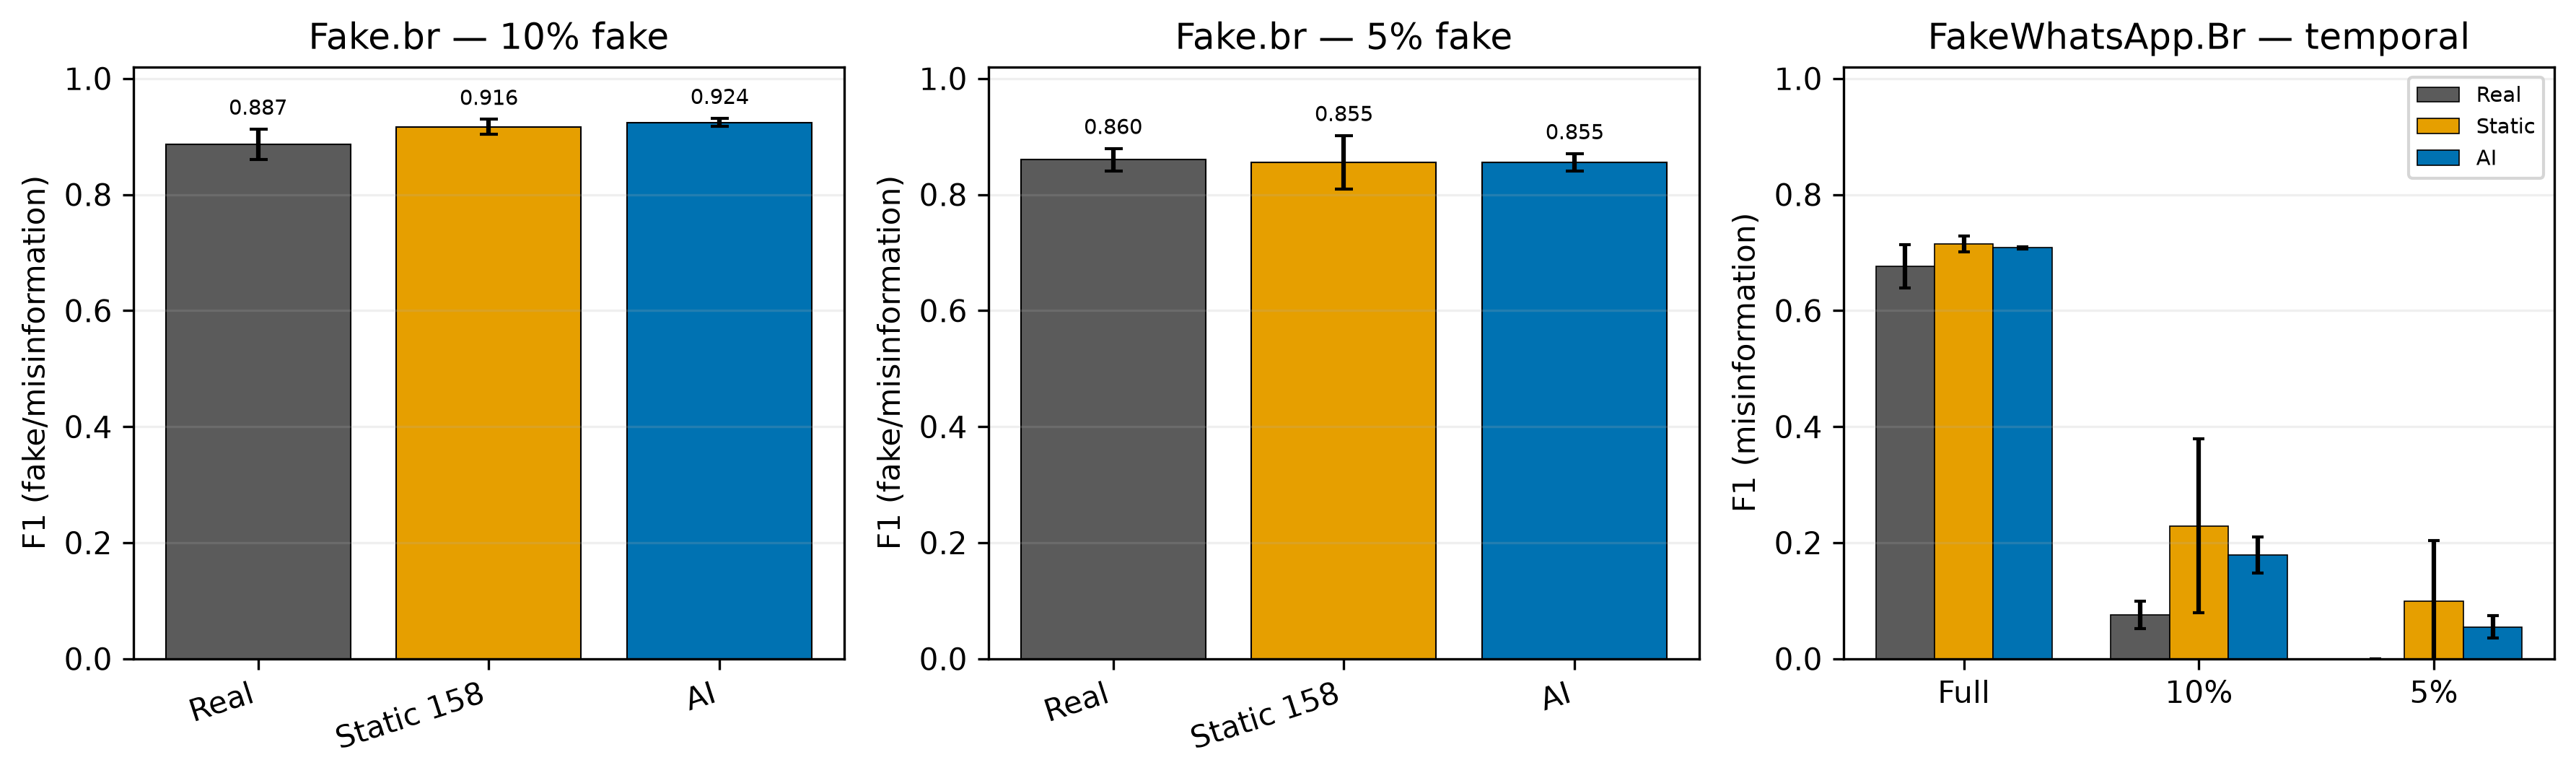
\includegraphics[width=.98\textwidth]{full_performance.png}
\caption{F1 nos experimentos principais. Barras mostram média e desvio em três seeds. ActiveInheritance lidera no Fake.br 10\%; Static lidera nos cenários temporais do FakeWhatsApp.Br.}
\label{fig:performance}
\end{figure*}

\section{Resultados no FakeWhatsApp.Br}

\begin{table}[t]
\caption{FakeWhatsApp.Br com split temporal e orçamento pareado ($\sim$100k tokens).}
\label{tab:wapp}
\centering
\resizebox{\columnwidth}{!}{%
\begin{tabular}{llrrr}
\toprule
Cenário & Braço & F1 & Precisão & Recall\\
\midrule
Full & Real & $0{,}676\pm0{,}037$ & 0,736 & 0,637\\
Full & \textbf{Static} & $\mathbf{0{,}715\pm0{,}014}$ & 0,668 & 0,774\\
Full & AI & $0{,}708\pm0{,}002$ & 0,727 & 0,691\\
\midrule
10\% & Real & $0{,}075\pm0{,}024$ & 0,885 & 0,040\\
10\% & \textbf{Static} & $\mathbf{0{,}229\pm0{,}150}$ & 0,799 & 0,148\\
10\% & AI & $0{,}179\pm0{,}032$ & 0,783 & 0,101\\
\midrule
5\% & Real & $0{,}000\pm0{,}000$ & 0,000 & 0,000\\
5\% & \textbf{Static} & $\mathbf{0{,}099\pm0{,}105}$ & 0,681 & 0,058\\
5\% & AI & $0{,}055\pm0{,}019$ & 0,764 & 0,029\\
\bottomrule
\end{tabular}}
\end{table}

O novo corpus é substancialmente mais difícil. No cenário full, Static possui maior média, mas AI fica apenas 0,007 abaixo e reduz fortemente a variância. AI usa somente 64 herdados contra cerca de 347 textos Static, indicando eficiência de dados de treino, mas ambos consomem o mesmo orçamento de geração.

Com 10\%/5\%, o learner colapsa para a classe majoritária. Precisão alta mascara recall de 4\% ou zero no Real. Static melhora recall por também rebalancear o treino por volume. AI herda poucos textos (64), insuficientes para compensar 683 negativos, e seu gate recebe sinal fraco do learner inicial. A Fig.~\ref{fig:recall} evidencia que escassez afeta sobretudo o recall.

\begin{figure}[t]
\centering
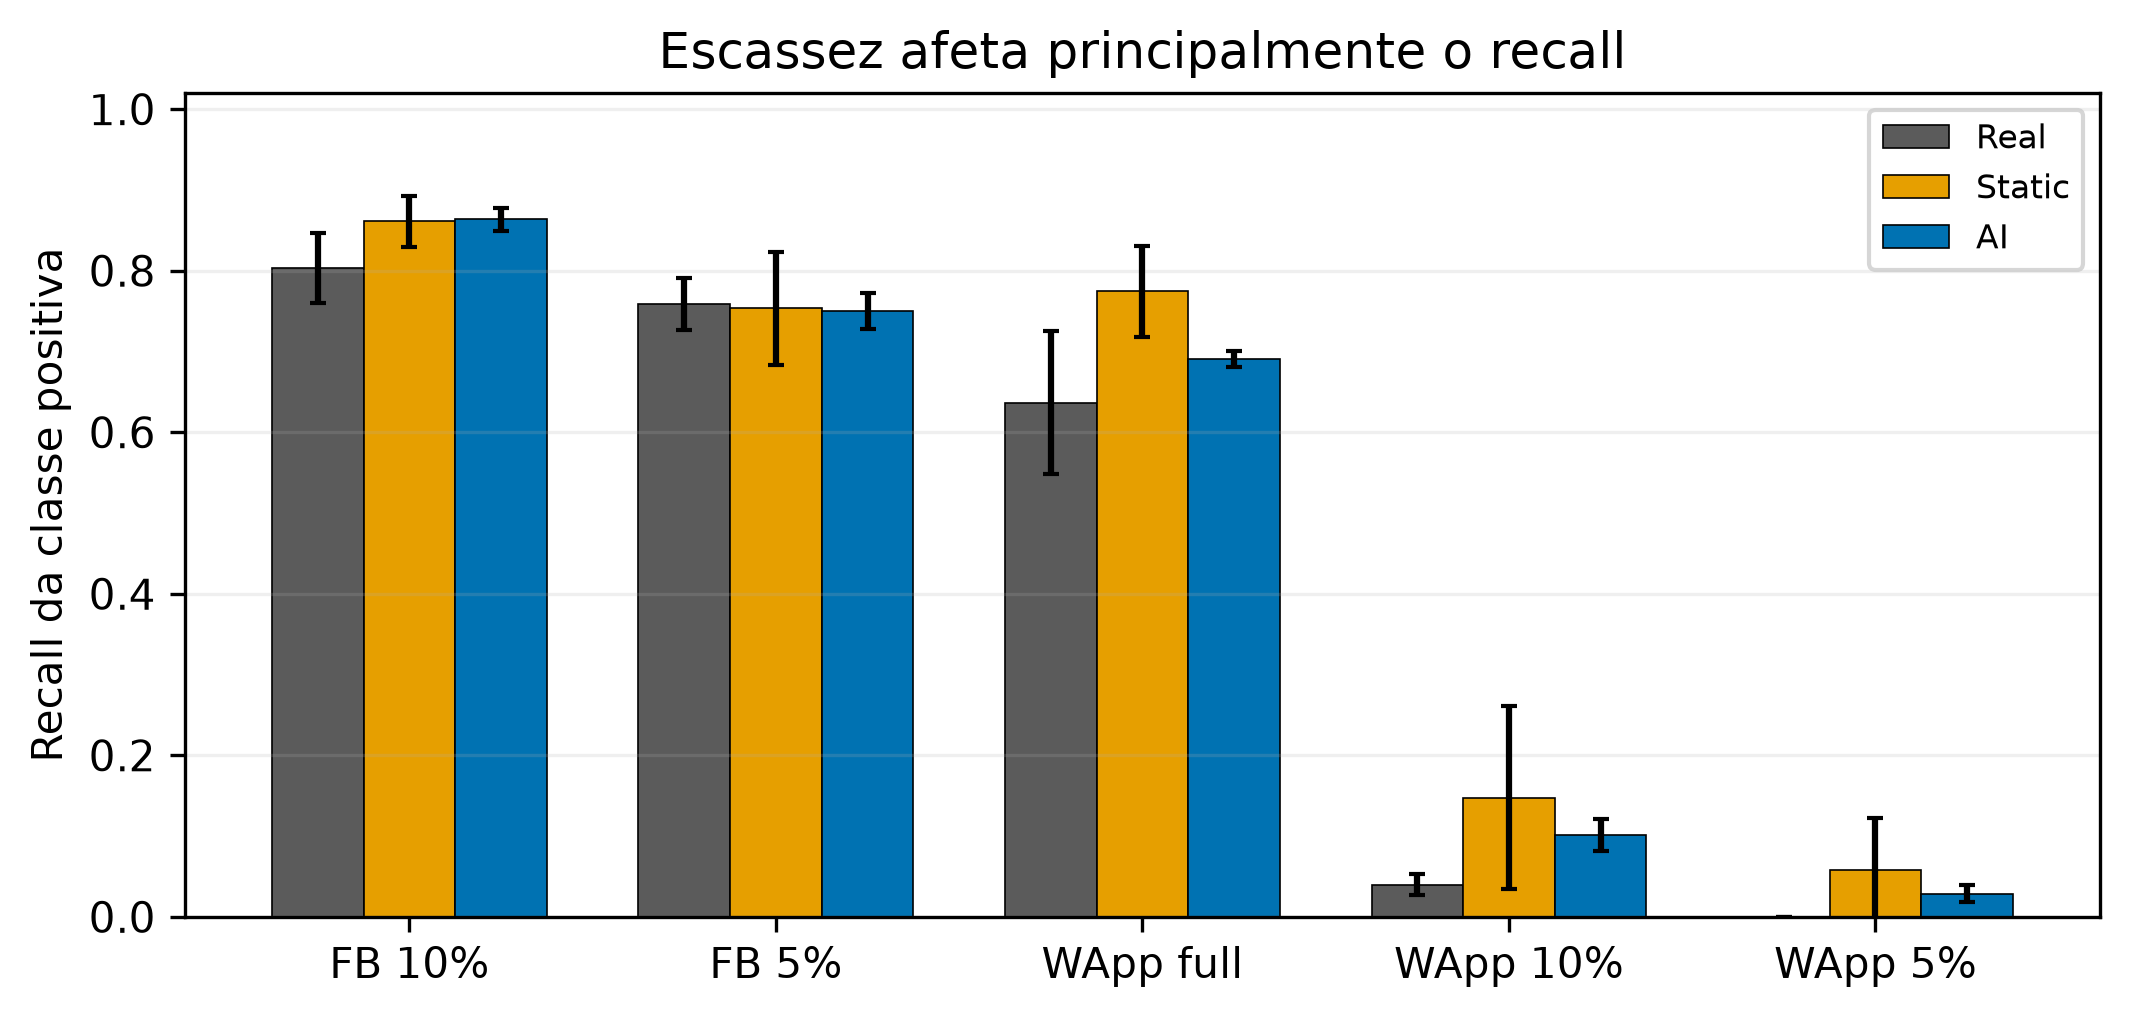
\includegraphics[width=\columnwidth]{full_recall.png}
\caption{Recall da classe positiva por corpus e nível de escassez. A queda extrema explica o F1 baixo no FakeWhatsApp.Br.}
\label{fig:recall}
\end{figure}

\section{Análise do Mecanismo}

\subsection{Saturação da Incerteza}

A Fig.~\ref{fig:uncertainty} mostra que a incerteza cai rapidamente após o primeiro ciclo. O learner aprende o estilo sintético e torna-se confiante; nos ciclos finais, o termo de entropia quase deixa de contribuir. A seleção passa a depender de erro relativo e diversidade. Isso explica platôs de validação e sustenta early stopping, ensemble/MC-dropout ou recalibração.

\begin{figure}[t]
\centering
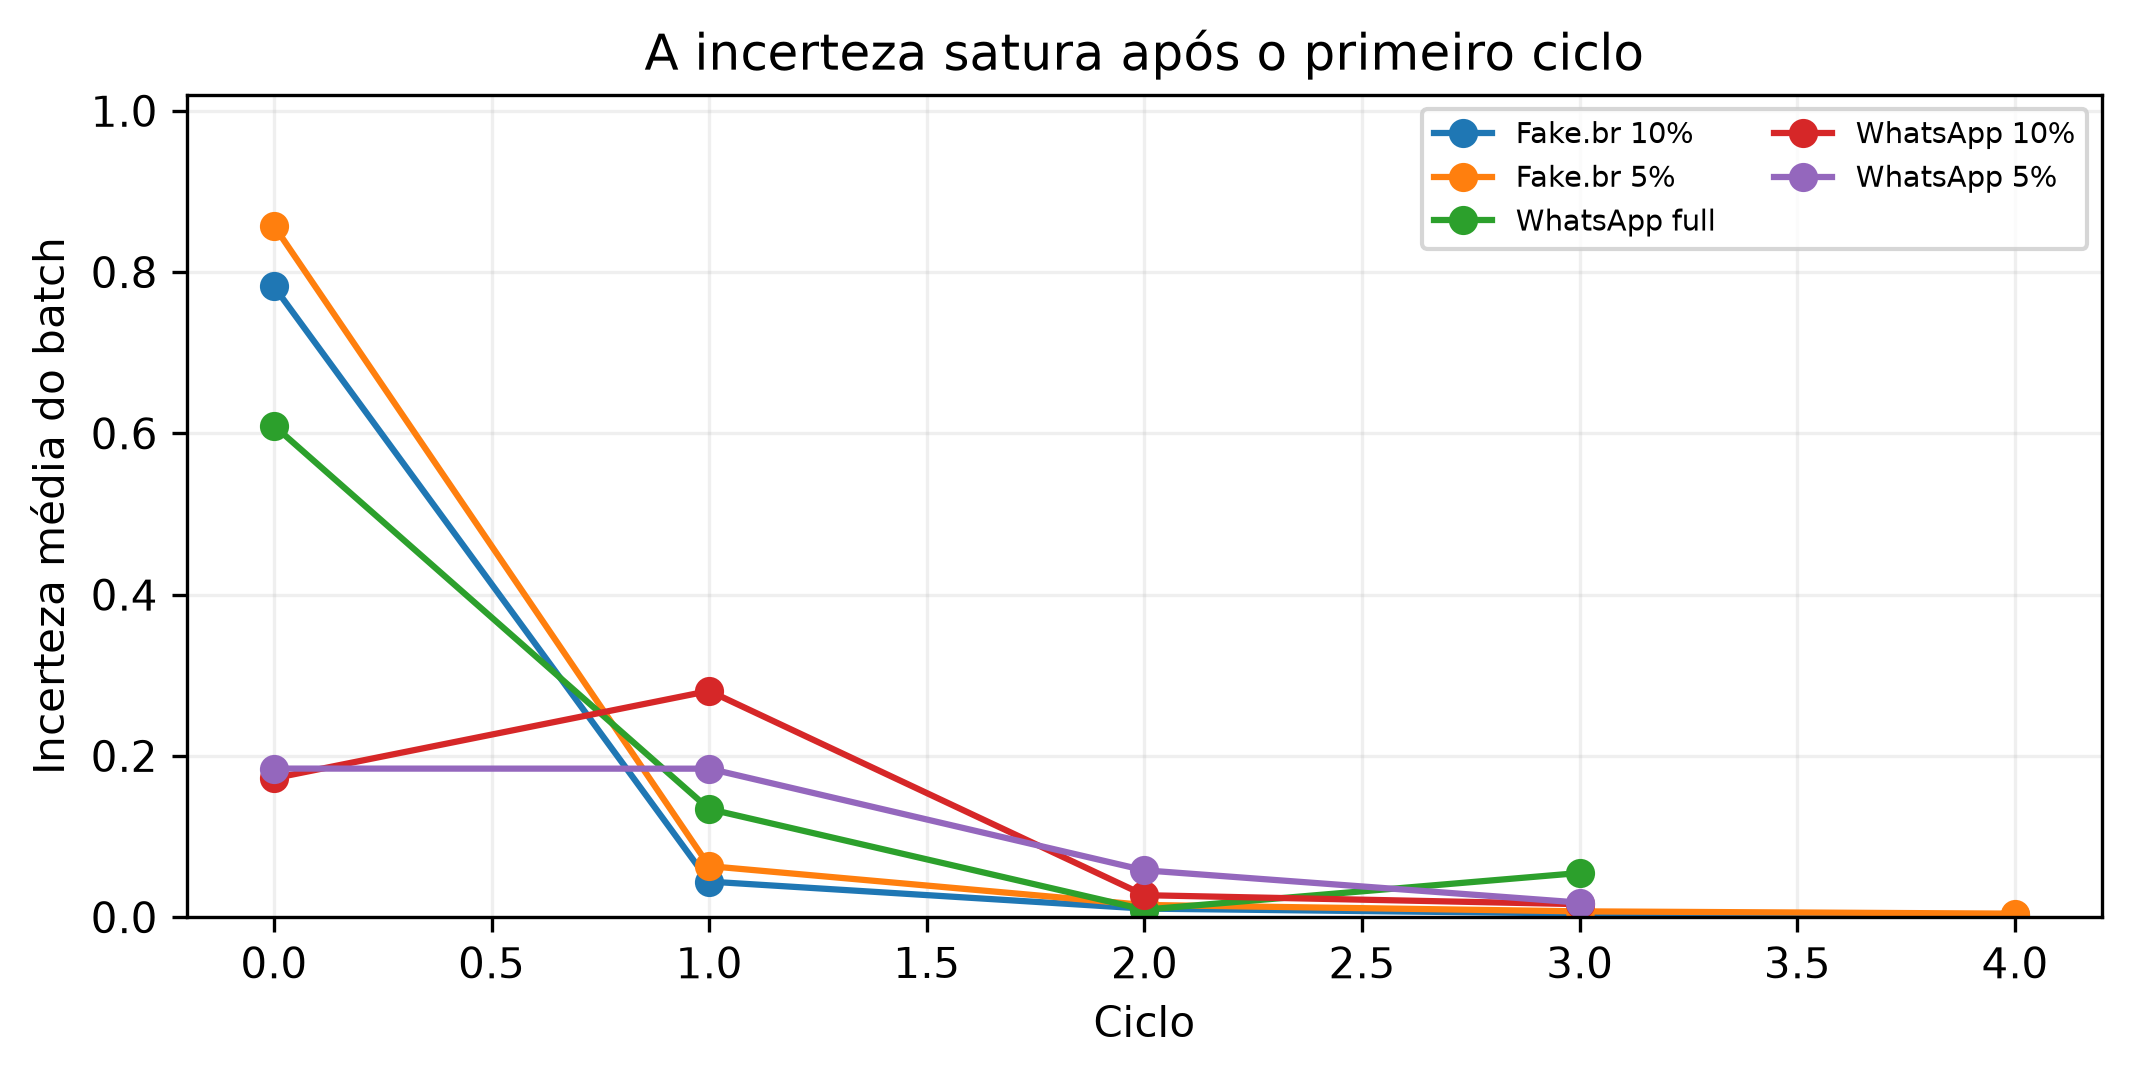
\includegraphics[width=\columnwidth]{full_uncertainty.png}
\caption{Incerteza média dos batches AI. Após o primeiro ciclo, o sinal satura em quase todos os cenários.}
\label{fig:uncertainty}
\end{figure}

\subsection{Diversidade versus Fidelidade}

A seleção de diversidade reduz repetição no pool, mas não garante realismo: distância de cosseno é calculada contra herdados, não contra dados reais. Wasserstein apenas avalia o resultado. Um candidato pode ser novo e ainda estar fora da distribuição. Esse problema aparece claramente no prompt WhatsApp.

\subsection{Colapso de Template}

Embora v3 elimine Markdown, recusas e duplicatas exatas, 91--93\% das gerações Static começam por ``URGENTE'' e 85--86\% contêm ``acabei de receber''; no real, aproximadamente 1\% e 0\%. AI reduz esses padrões a 29--36\%, mostrando filtragem parcial, mas não os elimina (Fig.~\ref{fig:templates}). Além disso, fake real tem média aproximada de 159 palavras, contra 95--100 nos sintéticos, limitados a 120. A Tabela~\ref{tab:quality} resume os proxies; TTR maior indica mais variedade lexical, enquanto similaridade e Wasserstein menores são preferíveis sob suas respectivas interpretações.

\begin{table}[t]
\caption{Qualidade do sintético no FakeWhatsApp.Br.}
\label{tab:quality}
\centering
\resizebox{\columnwidth}{!}{%
\begin{tabular}{llrrrr}
\toprule
Cenário & Braço & Pool sim. & TTR & Wasserstein & Palavras\\
\midrule
Full & Static & 0,413 & 0,598 & 0,162 & 99,7\\
Full & AI & 0,434 & 0,792 & 0,176 & 95,4\\
10\% & Static & 0,411 & 0,598 & 0,184 & 99,6\\
10\% & AI & 0,389 & 0,831 & 0,192 & 95,8\\
5\% & Static & 0,417 & 0,597 & 0,183 & 99,1\\
5\% & AI & 0,386 & 0,826 & 0,187 & 96,6\\
\bottomrule
\end{tabular}}
\end{table}

\begin{figure}[t]
\centering
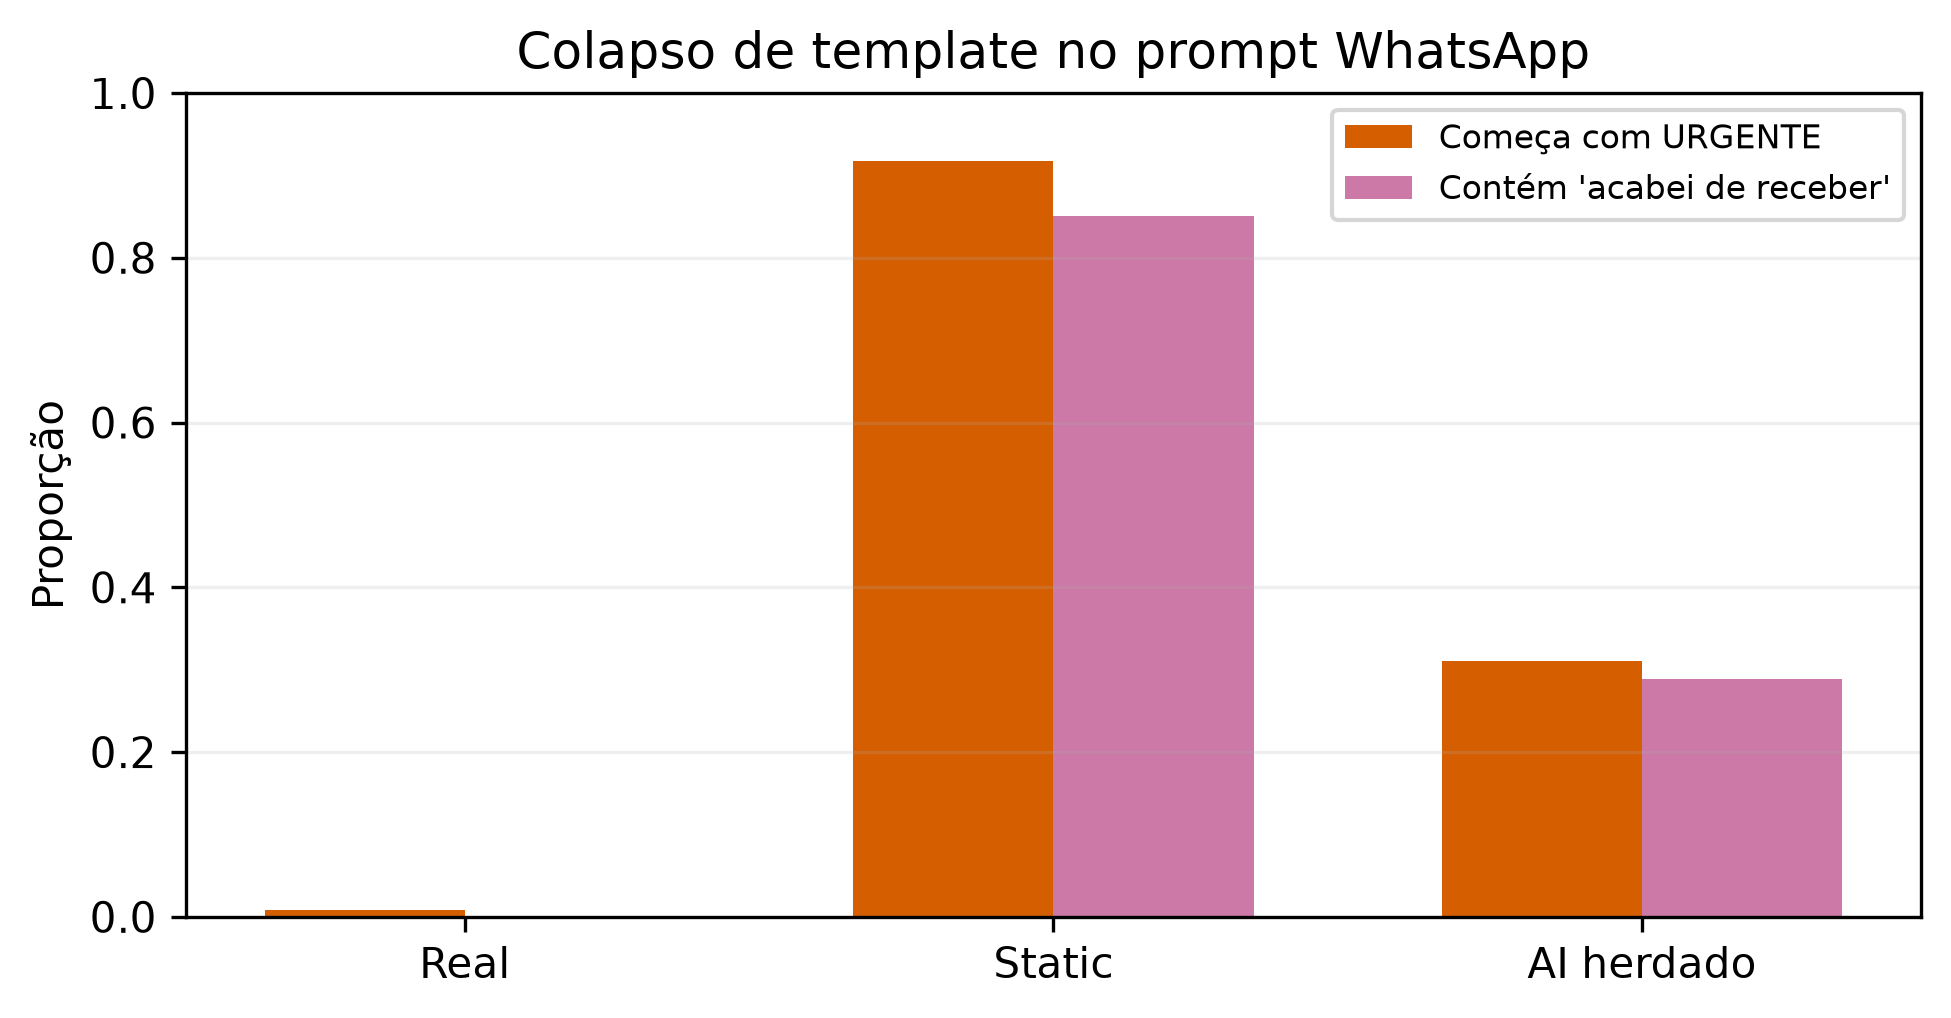
\includegraphics[width=\columnwidth]{full_templates.png}
\caption{Artefatos de template no FakeWhatsApp.Br. AI filtra redundância, mas permanece distante do real.}
\label{fig:templates}
\end{figure}

\section{Discussão}

\subsection{Por que AI funciona somente em alguns cenários?}

ActiveInheritance forma um ciclo de feedback: o learner escolhe exemplos que depois alteram o próprio learner. Quando a base inicial é forte, como no Fake.br 10\%, erro/incerteza são sinais razoáveis. Sob escassez severa, o learner prevê quase tudo como true; o gate passa a herdar seus vieses. Além disso, erro alto pode significar exemplo informativo, mas também outlier artificial, texto ambíguo ou rótulo presumido incorreto.

Static possui uma vantagem adicional: atua como rebalanceamento. No FakeWhatsApp 5\%, Real começa com 23 positivos/683 negativos; AI termina com 87 positivos (23+64), enquanto Static adiciona cerca de 347 e aproxima as classes. Isso explica recall médio maior, mesmo com sintéticos imperfeitos.

\subsection{O que foi e não foi confirmado}

Os dados apoiam parcialmente que AI:

\begin{itemize}
\item reduz variância entre seeds;
\item filtra templates e redundância;
\item alcança desempenho próximo ao Static com pool herdado menor;
\item funciona melhor quando o learner inicial é competente.
\end{itemize}

Não apoiam que AI:

\begin{itemize}
\item seja mais eficiente em tokens;
\item supere consistentemente geração estática;
\item resolva escassez extrema;
\item funcione com qualquer decision model zero-shot.
\end{itemize}

\subsection{Limitações}

Além do baixo número de seeds, rótulos sintéticos são assumidos como fake sem checagem factual humana. No Fake.br, real pré-processado e sintético raw podem criar atalhos. No FakeWhatsApp, usuários podem reaparecer temporalmente, embora ID não seja feature. O BERT não usa class weighting/sampler balanceado, confundindo qualidade sintética com política de treino. Veracidade factual pode exigir evidência externa, não apenas estilo. Métricas de embedding são proxies, e TTR depende do tamanho do conjunto.

\section{Próximos Passos}

Prioridades: (i) class weighting ou sampler balanceado no learner; (ii) prompt que amostre aberturas e comprimentos reais e evite templates dominantes; (iii) early stopping e orçamento pareado; (iv) ao menos 10 seeds nas comparações finais; (v) dados raw nos dois lados no Fake.br; (vi) validação humana de sintéticos; (vii) fine-tuning/calibração do decision model em treino/validação; e (viii) terceiro domínio, como COVID19.BR.

\section{Conclusão}

A hipótese de Herança Ativa foi parcialmente confirmada. No Fake.br 10\%, o método alcança maior F1 e menor variabilidade, porém com custo de tokens muito superior. No FakeWhatsApp.Br, Static apresenta maior média, enquanto AI é mais estável, filtra artefatos e obtém desempenho próximo com muito menos amostras herdadas. Sob 10\%/5\%, o baixo recall domina e nenhum método é operacionalmente satisfatório.

Assim, ActiveInheritance deve ser entendido como um mecanismo de \textbf{curadoria e estabilidade}, não como superioridade universal. Seu benefício depende de um learner inicial suficientemente competente, alinhamento entre distribuições real/sintética e um gerador sem templates dominantes. A implementação atual melhora consistência e reduz redundância, mas ainda não melhora eficiência de geração nem resolve escassez extrema.

\section*{Reprodutibilidade}

Foram preservados 60 JSONs oficiais em grupos separados, sem sobrescrita. Código, scripts, metadados e análises estão no repositório público\footnote{\url{https://github.com/Edu-p/active-inheritance-fraud}}. O protocolo completo e as análises detalhadas estão nos diretórios \path{docs/} e \path{planning/}. O FakeWhatsApp foi baixado com SHA-256 verificado; splits e contagens estão em \path{dataset/fakewhatsapp/metadata.json}.

\balance
\footnotesize
\begin{thebibliography}{00}

\bibitem{souza2025}
M.~D. de Souza and C.~Zanchettin, ``Breaking the Barrier of Hard Samples: A Data-Centric Approach to Synthetic Data for Medical Tasks,'' in \emph{Proc. ICML}, 2025.

\bibitem{monteiro2018}
R.~Monteiro, R.~Santos, T.~Pardo, T.~de Almeida, E.~Ruiz, and O.~Vale, ``Contributions to the Study of Fake News in Portuguese: New Corpus and Automatic Detection Results,'' in \emph{Proc. PROPOR}, 2018.

\bibitem{cabral2021}
L.~Cabral et al., ``FakeWhatsApp.Br: NLP and Machine Learning Techniques for Misinformation Detection in Brazilian Portuguese WhatsApp Messages,'' in \emph{Proc. ICEIS}, 2021.

\bibitem{souza2020}
F.~Souza, R.~Nogueira, and R.~Lotufo, ``BERTimbau: Pretrained BERT Models for Brazilian Portuguese,'' in \emph{Proc. BRACIS}, 2020.

\bibitem{shumailov2024}
I.~Shumailov et al., ``AI Models Collapse When Trained on Recursively Generated Data,'' \emph{Nature}, vol.~631, 2024.

\end{thebibliography}

\end{document}
